\documentclass{article}
\usepackage[a4paper, total={6.5in, 8in}]{geometry}
\usepackage[utf8]{inputenc}
\usepackage[T1]{fontenc}
\usepackage{hyperref}
\usepackage{polski}
\usepackage{float}
\usepackage{amsmath}
\usepackage{booktabs}
\usepackage{mathtools}
\usepackage{amsfonts}
\usepackage{amssymb}
\usepackage{graphicx}
\usepackage{cases}
\usepackage{minipage-marginpar}
\usepackage{parskip}
\usepackage{tcolorbox}
\title{3 etap}
\date{}
\begin{document}

% \[
    % \lim_{n \to \infty} n \left( \sqrt[7]{1 + \frac{5}{n}} -1 \right) = \frac{5}{7}
% \]

% \[
    % \lim_{n \to 0} \sqrt[n]{\sqrt{n+1} - n } = e^{- \frac{1}{2}}   
% \]

\section*{ZADANIE 1}
Skoro \(y^2 = 4x\), to \(x\in\mathbb{R}_{\geq 0}\). 



\begin{tcolorbox}[colback=red!5!white,colframe=red!75!black,title=Rozwiązanie]
    wowoowowoowowwowow OKEJ DZIĘKUJE!
\end{tcolorbox}

\section*{ZADANIE 2}

\section*{ZADANIE 3}
\begin{minipage}{0.6\linewidth}
    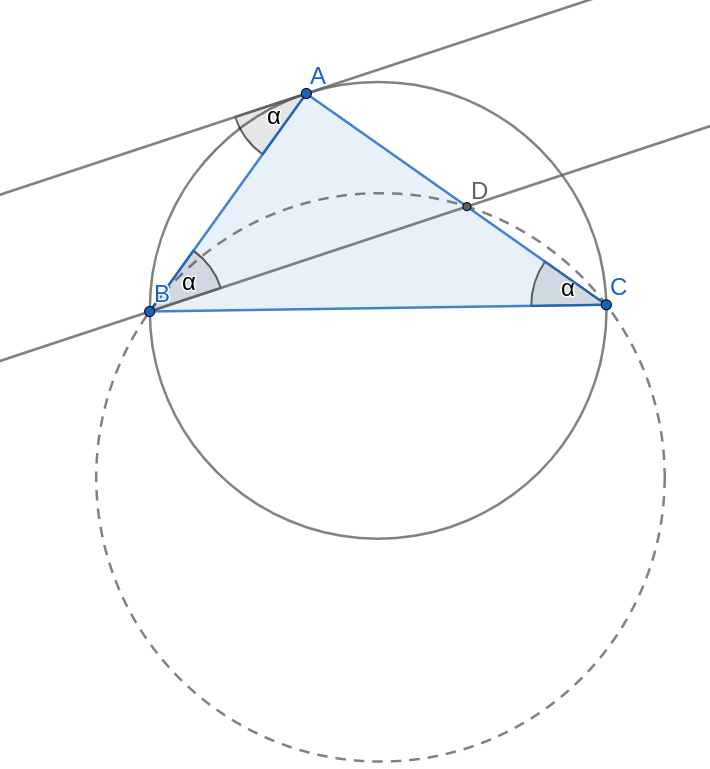
\includegraphics[width=\linewidth]{zadanie3pw.png}
\end{minipage}
\begin{minipage}{0.4\linewidth}
    Oznaczmy przez \(\alpha\) kąt pomiędzy odcinkiem \(AB\) a prostą styczną do okręgu opisanego na \( \triangle ABC \). Z własności kątów dopisanych i opisanych opartych na tym samym łuku \(AB\) wiemy, że \(\angle ACB = \alpha \). Ponadto z równoległości stycznej do prostej \(BD\) mamy, że \(\angle ABD = \alpha \). Opiszmy okrąg \(\omega\) na \(\triangle BCD\). Skoro \(\angle DBA = \angle DCB\), to prosta \(AB\) jest styczna do \(\omega\)  w punkcie \(B\). Rozważmy potęgę punktu \(A\) względem \(\omega\). Mamy, że \(AB^2 = AC \cdot CD\), co po spierwiastkowaniu stronami daje tezę. 
\end{minipage}

\[
    \left\lfloor 2\sqrt{n-\left\lfloor \sqrt{n}  \right\rfloor}  \right\rfloor + 1 \leq \left\lfloor 2\sqrt{n}  \right\rfloor
\]


\section*{ZADANIE 4}

get out\\
Założenia: \(0 <  \alpha , \beta < \pi \).\\
Teza: jeśli spełniona jest poniższe równanie, to trójkąt o dwóch kątach \(\alpha , \beta \) jest prostokątny.
\[
    1 + \cos ^2(\alpha +\beta ) = \cos ^2 \alpha  + \cos ^2\beta  %= [ \beta = \pi, \  \beta = - i \ln{(- e^{- i \alpha})}, \  \alpha = \pi, \  \alpha = - i \ln{(- e^{- i \beta})}]
\]
Przekształcając równoważnie:
\[
    \cos ^2(\alpha +\beta ) - \cos^2\alpha = \cos ^2 \beta -1
\]
\[
    (\cos (\alpha + \beta ) - \cos \alpha )(\cos (\alpha +\beta ) + \cos \alpha ) = \cos ^2 \beta - 1 = (1-\sin ^2 \beta ) - 1 = - \sin ^2 \beta 
\]
Wzorki, więcej wzorków:
\[
    (\cos (\alpha + \beta ) - \cos \alpha )(\cos (\alpha +\beta ) + \cos \alpha ) = -2 \sin \frac{2\alpha +\beta }{2} \cdot \sin \frac{\beta}{2} \cdot 2 \cos \frac{2\alpha +\beta}{2} \cdot \cos \frac{\beta}{2} = - \sin (2\alpha +\beta ) \sin \beta  = - \sin ^2 \beta 
\]
\[
    \sin (2\alpha +\beta ) \sin \beta  = \sin ^2 \beta 
\]
\[
    \sin \beta (\sin (2\alpha +\beta ) - \sin \beta ) = 0 \implies \sin \beta = 0 \lor \sin (2\alpha +\beta ) = \sin \beta 
\]
Wiemy, że \( \forall_{0 < \beta < \pi } \sin \beta  > 0\), zatem musi zachodzić:
\[
    \sin (2\alpha +\beta ) = \sin \beta 
\] 
Rozważmy dwa przypadki (bo założenia):
\begin{enumerate}
    \item \(2\alpha +\beta = \beta \), sprzeczność, bo wtedy \(\alpha = 0^{\circ}\).
    \item \(2\alpha + \beta + \beta = \pi \implies \alpha + \beta = \frac{\pi}{2} \implies \) trzeci kąt trójkąta będzie wynosić \(90^{\circ}\), co kończy dowód.    
\end{enumerate}

\section*{ZADANIE 5}
Rozważmy dwusieczną kąta \(\alpha \) wycinka. Z symetrii na tej dwusiecznej leży środek okręgu wpisanego w wycinek. Przez \(r\) oznaczmy promień okręgu wpisanego. Zatem:
GET OUT
\[
    \sin \left(\frac{\alpha}{2}\right) = \frac{r}{R-r} \implies r = R \frac{\sin (\frac{\alpha}{2})}{1 + \sin (\frac{\alpha}{2})}.
\] 

\section*{ZADANIE 6}

Oznaczmy to zdarzenie przez \(\mathcal{A}\). 
Wszystkich możliwości sześciu rzutów sześcienną kostką jest \( |\Omega| = 6^6\). Teraz: do dwóch pierwszych rzutów możemy na 3 sposoby wybrać liczbę oczek mniejszą niż 4, następnie spośród pozostałych 4 rzutów na \(\binom{4}{3} = 4\) sposoby możemy wybrać rzuty, które będą miały liczbę oczek równą co najmniej 4 (podczas każdego z tych rzutów może pojawić się liczba oczek równa \(\{4, 5, 6\}\) - na trzy sposoby). Ostatni rzut będzie liczbą ze zbioru \(\{ 1, 2, 3\}\), ponieważ dokładnie 3 rzuty miały liczbę oczek równą co najmniej 4. Zatem łączna liczba sposobów spełniających warunki zadania to:
\[
    3^2 \cdot 4 \cdot 3^3 \cdot 3 = 3^6 \cdot 4
\]
Czyli prawdopodobieństwo wynosi:
\[
    P(\mathcal{{A}}) = \frac{3^6 \cdot 4}{6^6} = \frac{1}{16}.
\]

\section*{ZADANIE 7}
Niech \(f(x) = x^5 + 5x-1\). Policzmy pochodną: \(f^\prime (x) = 5x^4 + 5 \implies \forall_{x\in\mathbb{R}} f^\prime (x) > 0\), zatem funkcja jest rosnąca w całej swojej dziedzinie. Zauważmy, że:
\(f(1) = 1+5-1=4\) oraz \(f(-1) = -1-5-1=-7\). Z własności Darboux wielomianów istnieje dokładnie jeden \(x\in(-1, 1)\), że \(f(x) = 0\). 


\section*{ZADANIE 8}

\begin{enumerate}
    \item \(f(x) = y = \frac{x^2 - 4x + 3}{x^2 + 4x + 3}\)
    \[
        f^\prime(x) = \frac{(x^2 - 4x + 3)^\prime (x^2 + 4x + 3) - (x^2 - 4x + 3)(x^2 + 4x + 3)^\prime }{(x^2 - 4x + 3)^2} = 
    \]
    \[
        = \frac{(2x-4)(x^2 + 4x + 3) - (x^2 - 4x + 3)(2x+4)}{(x^2 + 4x + 3)^2}  = \frac{8 (x^{2} - 3)}{(x^2 - 4x + 3)^2}
    \]
    Dziedzina hshsh.
    \[
        f^\prime (x) = 0 \iff 8(x^2 - 3) = 0 \iff  x \in \{ -\sqrt{3}, \sqrt{3} \} 
    \]

    \item \(g(x) = y = \frac{x\sqrt{x} }{1-x}\) 
    \[
        g^\prime (x) = \frac{(x\sqrt{x} )^\prime (1-x)-(1-x)^\prime (x\sqrt{x} )}{(1-x)^2} = \frac{\frac{3}{2}\sqrt{x} (1-x) + x\sqrt{x} }{(1-x)^2}  = \frac{\sqrt{x} (3 - x)}{2 (x - 1)^{2}}
    \]
    \[
        g^\prime (x) = 0 \iff \sqrt{x} (3-x) = 0 \iff x \in \{0, 3\}.
    \]
\end{enumerate}

\section*{ZADANIE 9}

Wzór na sumę piątych potęg pierwszych \(n\) liczb naturalnych wyraża się wzorem:
\[
    S_n = \frac{n^2(n+1)^2 (2n^2 + 2n - 1)}{12}
\]
Udowodnijmy go indukcyjnie. Baza indukcji: \(n = 1\): \(S_1 = \frac{1\cdot 2^2 \cdot (2 + 2 - 1)}{12} = \frac{12}{12} = 1\). Krok indukcyjny - załóżmy, że dla pewnego \(k \in \mathbb{Z}_+\) wzór ten jest spełniony. Rozważmy teraz
\[
\sum_{i=1}^{k+1} i^5 = \sum_{i=1}^{k}i^5 + (k+1)^5 =  \frac{k^2(k+1)^2 (2k^2 + 2k - 1)}{12} + (k+1)^5 = \frac{(k+1)^2(k^2(2k^{2}+2k-1)+12(k+1)^3)}{12} = 
\]  
\[
    = \frac{(k+1)^2 (2k^4 + 14k^3 + 35k^2 + 36k + 12)}{12} = \frac{(k+1)^2(k+2)^2(2k^2+6k+3)}{12} =
\]
\[
    =\frac{(k+1)^2(k+2)^2(2(k+1)^2 + 2(k+1)-1)}{12},
\]
co kończy dowód indukcyjny. Zatem
\[
    S_{2021} = \sum_{i=1}^{2021} i^5  = \frac{2021^2\cdot 2022^2 \cdot (2\cdot 2021^2 + 2 \cdot 2021 - 1)}{12} = (43 \cdot 47)^2 \cdot \frac{2022}{6} \cdot \frac{2022}{2} \cdot 8172923 = 43^2 \cdot 47^2 \cdot 337 \cdot 3 \cdot 337 \cdot 11 \cdot 742993 
\]
\[
    S_{2021} = 3 \cdot 11 \cdot 43^2 \cdot 47^2 \cdot 337^2 \cdot 742993.
\]

\end{document}

